\documentclass[letterpaper]{article}
\usepackage{aaai}
\usepackage{times}
\usepackage{helvet}
\usepackage[colorlinks]{hyperref}
\usepackage{courier}
\usepackage{graphicx}
\usepackage{float}
\frenchspacing
\setlength{\pdfpagewidth}{8.5in}
\setlength{\pdfpageheight}{11in}
\setcounter{secnumdepth}{0}
\begin{document}

\title{Amazon Reviews - classification of a multi-class  dataset}
\author{Artur Juraszek}
\maketitle

\section{Project goal}
The dataset being the center of this project is a small-ish (about 1.5 GB) subset of reviews produced by
Amazon users throughout the last two decades.
It, among other things which this time are of no interest to us, contains two types of data - an overall
rating, in form of 1 to 5 stars, which, as one could guess, represent the given user's attitude into
a particular product, and, more importantly, a (usually) short corresponding text, consisting of
the user's review written in English. The main question we would like to ask is: \textbf{Knowing the 
review's text content, can we predict which 1 to 5 stars rating it gives?}

\section{Overview of the dataset}
The review database, \href{http://jmcauley.ucsd.edu/data/amazon/}{provided
through courtesy of Julian McAuley from UCSD} stores exactly 1,697,533 records taken from
\textit{Movies and TV} Amazon's store category. Unfortunately, it's extremely unevenly
distributed - 5 stars ratings account for the vast majority of it, and 2 'lowest' classes
are visibly underrepresented.

\begin{figure}[h]
    \centering
    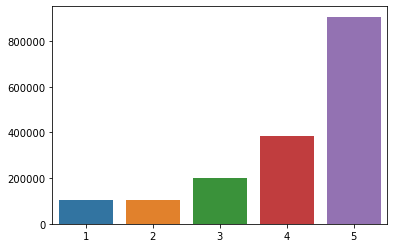
\includegraphics[scale=0.5]{dataset-distribution.png}
    \caption{Class distribution, 1 to 5 stars}
\end{figure}

An arbitrarily split has been made, to 75\% of data being a training sample and another 25\% - a testing set,
keeping their uneven distribution the same as the full dataset.

\begin{figure}[t]
    \centering
    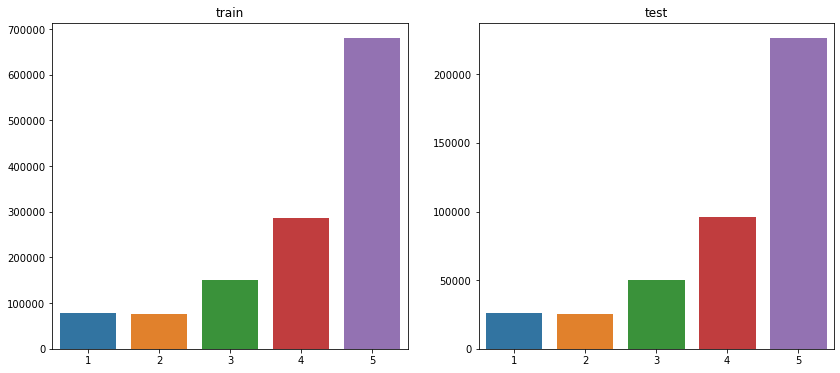
\includegraphics[scale=0.3]{train-test.png}
    \caption{Shard's distribution has been preserved}
\end{figure}

Three approaches has been leveraged to tackle this balance problem:

\begin{itemize}
    \item Keeping the class proportions unchanged
    \item Discarding some arbitrary data from overrepresented classes, i.e. randomized undersampling, presented below
    \item Augmenting the training dataset in form of copying the minor-iest classes a few times
\end{itemize}

\begin{figure}[h]
    \centering
    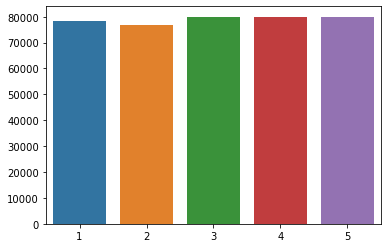
\includegraphics[scale=0.5]{downsampling.png}
    \caption{Class distributions after randomized downsampling}
\end{figure}

\section{Classification accuracy measure}
Due to dataset's imbalance, the tempting thought to use the simple percentage-based accuracy score as a measure
to compare classifiers on might in reality be not the best one - a smart, but not so much correct hypothetical model
could strongly favor the 5-star class and score higher than more 'smooth' ones, in extreme case, even by always predicting '5'.

To mitigate this risk, a so called \textbf{balanced accuracy score} has been used, defined as an average of single-class accuracies.
A custom metric measuring serioussness of the errors was also calculated - due to classes having a trivial
order defined on them (1 $>$ 2, 5 $>$ 3 and so on) one could reason about the errors being made
in terms of averaged distance of the error, namely:
\[ orderedErr(class) = \frac{\Sigma \mid pred_i - true_i \mid}{\# classifiedIncorrectly} \]
Where \textit{i} are samples which belong to class \textit{class}.

Measuring area under the \textbf{Receiver Operating Curve} looked promising too, but due to apparent lack of consensus on
which flavor of it (1 vs 1 or 1 vs rest) should be used in a multi-class scenario, it has been left alone.

\section{Text preprocessing}
Three methods has been tried:
\begin{itemize}
    \item Keeping the data dirty
    \item So-called "stop words" removal
    \item Stemming, in simple words removing the word suffixes introduced by English language's  inflection,
    so, for example 'fishing' and 'fisher' both end up in the same bucket, namely 'fish'
\end{itemize}
Another popular technique, foreign accents removal was immediately discarded, as the data had already been
represented as 7-bit ASCII, so no room for improvement (or the opposite, possibly) here.
Also, after initial experimentation (with Naive Bayes approach, in belief that it will be representative
enough to deduct anything from these manual experiments) it turned out that stop-words removal based on
popular 'stop-word lists' showed no improvement, and in most (all) cases produced worse results than the
dirty data alone. This can be explained by appearance of words such as "however" in this lists,
which in our case would probably suggest that the review author has some "BUT" - thus indicating this review is not a 5-star one.
To avoid combinatorial explosion of methods being used on not-so-fast hardware,
it has thus been discarded too.

\section{Word representation}
Again, three vectorization approaches has been tried:

\begin{itemize}
    \item Treating text chunk as a position independent vector of word occurences in it - reviews span rows,
    words used across the whole training dataset make up columns
    \item A small twist to the method above - ignoring word repetitions, i.e. storing either 0 or 1
    instead of a proper occurence count
    \item Popular TF-IDF, more or less a transformation in which we replace word/term occurence counts
    with a product of \textbf{t}erm \textbf{f}requency and \textbf{i}nverse \textbf{d}ocument \textbf{f}requency -
    i.e. information how often the word/term occurs in the document (review) is "divided" by
    information on how often it is across the whole dataset
\end{itemize}
Note that words not necessarily mean words here, they could as well be N-grams and in fact are,
in experiments conducted on best-promising estimators.

\section{Baseline estimator}
A really dumb, randomly guessing classifier has been prepared as a baseline for other estimators.
Not surprisingly, it can be summed up with:

\begin{itemize}
    \item Balanced accuracy of \textbf{about 20\%}
    \item "Real-world" accuracy, not taking class distribution into account
    (from now one we will refer to it via similar expressions) of \textbf{35.645\%}
    \item Very heavy bias towards classes 5 or 4 - the overrepresented ones.
    Easily noticable on the confusion matrix provided below.
\end{itemize}

\begin{figure}
    \centering
    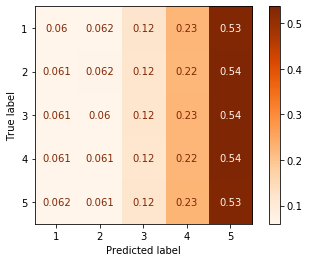
\includegraphics[scale=0.9]{baseline-confusion-matrix.png}
    \caption{Confusion matrix of the baseline estimator}
\end{figure}

\section{Naive Bayes}
First classification technique tried was Naive Bayes - a few nested loops were ran, resulting in
the cartesian product of two sampling methods (randomized downsampling and untouched dataset),
two word representations, either stemming usage or not preprocessing the data at all, and last, but
not least - two hyperparameters to NB, specifically \textbf{alpha} and a boolean of whether
prior probabilities assigned to classes should be uniform, or deducted from the training dataset.

\paragraph{}
Results were sorted on two independent conditions - a) balanced accuracy, b) real-world accuracy\\
A clear supremacy of \textbf{TF-IDF} representation could be observed when evaluated by balanced acc,
among top 100 estimators, 84 were using this representation.
Surprisingly enough, it turned out to be the opposite after sorting by real-world acc - all 100 of top 100
estimators were based on simple count-based vectorization.

\par Similar correlation was observed in the matter of training dataset -
100 out of top 100 balance-acc-sorted
estimators were trained on either the randomized,
forcefuly balanced downsampled dataset or the oversampled one, while 100 out of 100
real-world-acc sorted ones were trained on the full, untouched dataset.
This \textbf{can be easily explained - exploiting the class imbalances, which are better reflected in the
"raw" training set will lead to higher real-world accuracies} (and probably the opposite for balanced-acc).
No significant value in having the input text stemmed was observed, thought no negative effect, neither -
stemmed and non-stemmed classifiers were interleaved among the top ones.\\
Best of the achieved results was:

\begin{itemize}
    \item For the balanced-accuracy-proritizing estimator,
    \textbf{47.3654\%} balanced accuracy with \textbf{48.8517\%} of real-world, biased accuracy.
    
    Averaged order-aware errors:
    \textbf{\#1: 1.619118, \#2: 1.246848, \#3: 1.309533, \#4: 1.316007, \#5: 1.673930, AVG: 1.433087}
    
    With \textbf{alpha = 0.5}, randomly downsampled training set, no preprocessing and \textbf{TF-IDF}
    \item For the real-world-prioritizing estimator, \textbf{40.7792\%} balanced, \textbf{60.3153\%}
\end{itemize}

Their confusion matrices are presented below.

\begin{figure}[H]
    \centering
    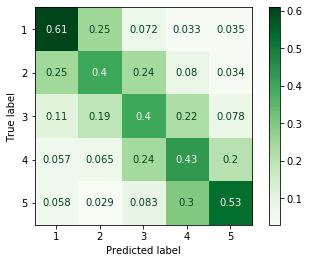
\includegraphics[scale=0.65]{naive-bayes-best-balanced.png}
    \caption{Naive Bayes winner when estimators are rated via their balanced accuracy, note the more even accuracies}
\end{figure}

\begin{figure}[H]
    \centering
    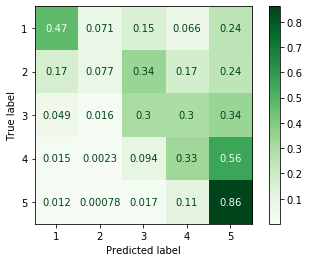
\includegraphics[scale=0.65]{naive-bayes-best-real-world.png}
    \caption{Strongly biased, bias-blind accuracy winner}
\end{figure}

In the perfect world, it would be easy to find a good compromise between these two accuracies, however, as presented
below, the dependencies are not that straightforward.

\begin{figure}[h]
    \centering
    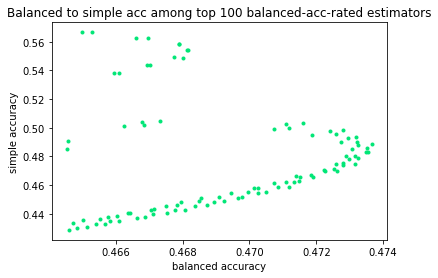
\includegraphics[scale=0.5]{naive-bayes-balanced-to-simple.png}
    \caption{Balanced to simple accuracy}
\end{figure}

\begin{figure}[h]
    \centering
    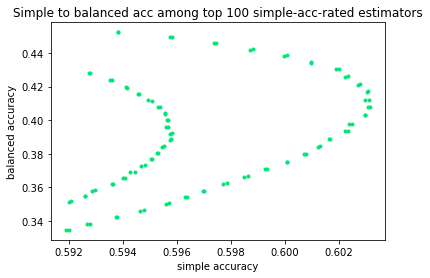
\includegraphics[scale=0.5]{naive-bayes-simple-to-balanced.png}
    \caption{Simple to balanced accuracy}
\end{figure}

\section{Logistic Regression}
Next, a linear approach in the form of Logistic regression was tried.
Same algorithm-independent parameter variations as in Naive Bayes trial has been set, in addition two
them, two log-regression specific hyperparameters were also included in the grid search -\textbf{ C}, a regularization
parameter, in theory preventing the model from overfitting and \textbf{mc}, the approach to generalizing log-regression
to multiclass scenario, taking one of two values - we either train one binary classifier per every class, i.e.
leverage a One-vs-Rest method or consider the model being multionmial and train over all classes at once.

Due to hardware constraints, optimization process lying underneath the algorithm was set to stop after 100 iterations,
regardless of how much has it really converged - however, even with that constraint the log-regression approach
proved better than Naive Bayes. Also, the 10 highest scoring hyperparameters combinations
were re-trained with a much higher limit of 1,000 iterations.

Again, TF-IDF representation proved to behave better than simple counting - when the result list has been
sorted by estimators performance, tf-idf based ones accounted for nearly half of the top results.

Also, One-vs-All approach had better results on average than Multinomial.

Two best classifiers on 100 iterations:

\begin{itemize}
    \item Balanced accuracy of \textbf{53.7067\%}, standard accuracy of \textbf{59.4022\%} 
    (\textbf{C = 0.05, stemming, One-vs-All, TF-IDF, oversampled training set})
    \item Balanced accuracy of \textbf{51.9371\%}, standard accuracy of \textbf{60.3992\%}
\end{itemize}

And the best on 1000 loops iteration limit, surprisingly, having all of the hyperparameters the same
as the 100-iterations winner with the exception of doing Multinomial instead of OvR multiclassing,
which actually stopped after 545 loops:
\begin{itemize}
    \item Balanced accuracy of \textbf{53.8411\%}, standard accuracy of \textbf{58.8100\%}
    
    Averaged order-aware errors:
    \textbf{\#1: 1.663587	\#2: 1.231656	\#3: 1.275698	\#4: 1.214740	\#5: 1.614087	AVG: 1.399954}
\end{itemize}

So the variation between these two metrics in best-predicting estimators is much, much less than before, in Naive Bayes.
Thus, choosing the top 1 instance would not result in such a big  tradeoff.
Picture below illustrates the regularization parameter's behavior on estimators class chosen as best on average.

\begin{figure}[H]
    \centering
    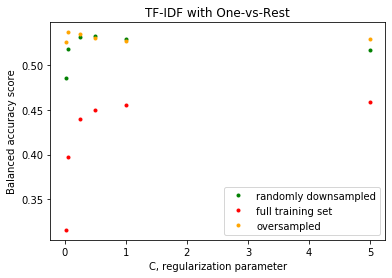
\includegraphics[scale=0.7]{logreg-behavior.png}
    \caption{Regularization parameter behavior}
\end{figure}

\begin{figure}[H]
    \centering
    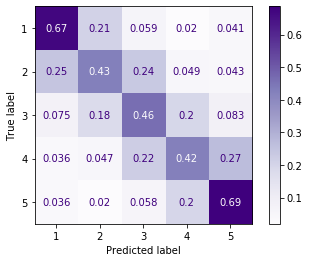
\includegraphics[scale=0.65]{logreg-before.png}
    \caption{Best Logistic Regression estimator (when rated with balanced accuracy)}
\end{figure}

\begin{figure}[H]
    \centering
    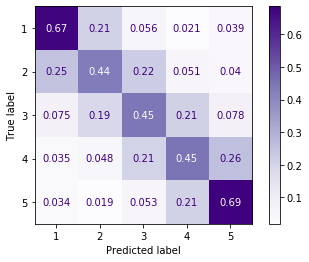
\includegraphics[scale=0.65]{logreg-after.png}
    \caption{Best Logistic Regression estimator (when rated with balanced accuracy, retrained with 545 iterations)}
\end{figure}

\begin{figure}[H]
    \centering
    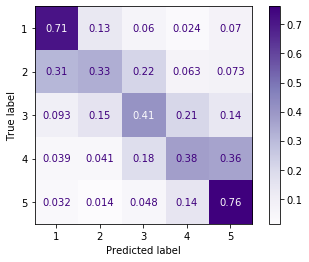
\includegraphics[scale=0.65]{log-regression-best-simple.png}
    \caption{Best estimator when rated with simple accuracy. Note the higher bias towards extreme classses}
\end{figure}

\section{AdaBoost}
Last of the three methods applied was AdaBoosting, an ensemble technique built on one-level decision trees
(aka \textit{stumps}).
An arbitrary number of estimation levels was assumed to be 10, and three different learning rates were tried.
Then, the best behaving hyperparameters combination was retrained with 1,000 levels of boosting.

\begin{itemize}
    \item Best: balanced accuracy = \textbf{33.9933\%}, simple accuracy = \textbf{42.9667\%},
    trained on the oversampled training set
    \item Most promising combination after retraining = \textbf{51.0199\%}, simple accuracy = \textbf{57.0877\%},
    
    Averaged order-aware errors:
    \textbf{\#1: 1.830312,	\#2: 1.277904,\#3: 1.316928,	\#4: 1.227841,	\#5: 1.716943,	AVG: 1.473986}
    \item Best on simple accuracy: balanced = \textbf{27.2546\%}, simple = \textbf{54.5826\%},
    trained on the full training set
\end{itemize}

Even though the simple accuracy metric is not \textit{that} bad, it's far worse than the previous two - 
the heavy bias towards class 5 almost mimics the dataset distribution, so the actual results are barely better than
a completely random estimator.

\section{Conclusions}
As expected, a strong bias towards classes 1 and 5 has been observed - it is probably easiest to detect extremities,
as some specific words tend to appear in them - e.g. "splendid" will probably not occur in 1-star review full of curses,
and the opposite would hold true for "crap".
That, however, might suggests good results in a simpler, 2-class (either 1 or 5) classification task - even with
the absolute imbalance between samples count the algorithms managed to do a proper separation.

\begin{figure}[h]
    \centering
    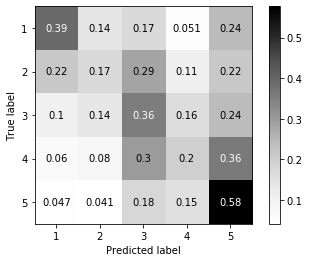
\includegraphics[scale=0.65]{adaboost-best.png}
    \caption{Best AdaBoost-based estimator}
\end{figure}

\begin{figure}[h]
    \centering
    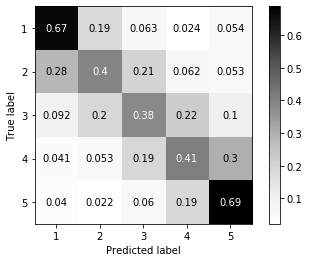
\includegraphics[scale=0.65]{adaboost-absolute-best.png}
    \caption{Best AdaBoost-based estimator}
\end{figure}

\begin{figure}[h]
    \centering
    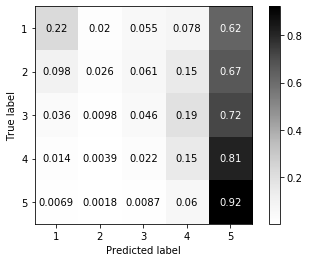
\includegraphics[scale=0.65]{adaboost-best-simple.png}
    \caption{"Best" AdaBoost-based estimator}
\end{figure}

\begin{figure}[h]
    \centering
    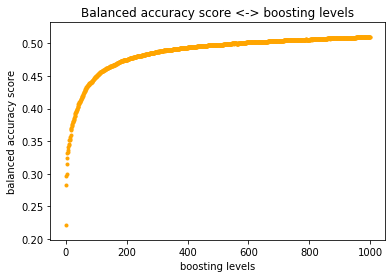
\includegraphics[scale=0.8]{adaboost-increase.png}
    \caption{AdaBoost accuracy increase}
\end{figure}

\end{document}